%ha med dette her
\documentclass[titlepage]{article}
\usepackage[english]{babel}
\usepackage[utf8]{inputenc}
\usepackage{parskip}
\usepackage{multirow}
%\usepackage[latin1]{inputenc}
\usepackage{graphicx}
\usepackage{float}
\usepackage{caption}

%---- Listings --------------
\usepackage{color}
\definecolor{light-gray}{gray}{0.95}
\usepackage{listings}
\lstset{numbers=right,
      %numberstyle=\tiny,
      %numbers=left,
      %stepnumber=2,
      literate={æ}{{\ae}}
        {Æ}{{\AE}}1
        {ø}{{\o}}1
        {Ø}{{\O}}1
        {å}{{\aa}}1
        {Å}{{\AA}}1,
      firstnumber=1,
      numberfirstline=true
     breaklines=true,
     backgroundcolor=\color{light-gray},
     numbersep=5pt,
     xleftmargin=.25in,
     xrightmargin=.25in}
     \lstset{language=Java}

%Listings brukes slikt:
%\begin{lstlisting}{insert}
%Sett inn kode her
%\end{lstlisting}
%--------------------------

%hva som skal stå på tittelsida
\author{Juul Arthur Ribe Rudihagen and Tobias Linkjendal}
\title{Exercise 3}
\date{\today}

\begin{document}

%lager forsida
\maketitle

%\renewcommand{\abstractname}{Summary}
%man burde ha med et sammendrag
%\begin{abstract}
%Sammendrag av rapporten
%\end{abstract}

%man skal ha romertall på de innholdsfortegnelse
%før dette punktet skal man IKKE ha sidetall
\pagenumbering{roman}
\tableofcontents

%newpage gjør at du starter på neste side etterpå
\newpage

%herfra skal vi ha vanlige tall (arabiske (1,2,3,4,5...))
\pagenumbering{arabic}

%man pleier å starte med innledning
\section{Deciding what to model}
We have chosen to model the decisions you can do when playing the computer game Smite. Smite is a MOBA (Multiplayer online battle arena) game where players cooperate and compete with each other over internett. Each game has 10 players, called gods, where 5 players are on each team. The goal of the game is to defeate the enemy gods and destroy their base. More specifically we have chosen the to model the decision of one of these players, when figthing against the other players. The question the player asks himself is "what should I do now?".

There are a lot of possibillities to do, and way to many variables to model. So we have limited this task to model only specefic parts of the game, and only take into consideration limited information. There are a lot of teamwork that can be done in this game, but we have choosen not to model this. We focus on the battle between us and one enemy god, and only model the other enemy as a group that can come and attack us.


\section{Defining variables and decisions}

\subsection{Variables}
\subsubsection{Certain variables}

\subsubsection*{Health}
How much health do I have?

\subsubsection*{EnemyHealth}
How much health do my enemy have?

\subsubsection*{UltimateAttack}
Can I use my ultimate attack? This is a skill that is not always available and I might not have it active, but it is the skill I have that deals the most damage.

\subsubsection*{AlliedMinions}
Do I have minions with me that will attack my enemy? Minions are weak computer-controlled characters that attacks the enemy minions and gods.

\subsubsection*{EnemyMinions}
Do my enemy have minions that will attack me?



\subsubsection{Uncertain variables}

\subsubsection*{EnemyAttack}
Will the enemy attack? This is dependent on our health, the enemy's health and our minions. The stronger the enemy is and the weaker we are, the greater is the chance that he will attack.

\subsubsection*{EnemyUltimate}
Will the enemy use its ultimate attack? If I have little or medium health the enemy is more likely to use his ultimate in order to kill me. If the enemy has little health he is also more likely to use his ultimate in order to kill or stun me before I am able to kill him.

\subsubsection*{Ganked}
Will I be attacked my multiple enemies? This is dependent on my health and whether I have allied minions or not, because the weaker I am the easier I am to gank/be killed.

\subsubsection*{Survive}
It is not desirable to die. When you die you lose gold, give the enemy more experience and gold. You also leave your team more vulnarable while you are dead. If you have little health and are weaker than your enemy you have to be very careful not to die. This also means that you are more likely to retreat if you are close to death.

\subsubsection*{KillEnemy}
It is very desirable to kill the enemy. This will leave you stronger and the enemy will be weaker. There is a risk though going for a kill, because you can easily get killed yourself.

\subsubsection*{GetGold}
To get gold is crucial to win the game, the more gold you have the stronger your god becomes. You get gold by killing minions and attacking the enemy.


\subsection{Decisions}

\subsubsection*{Attack}
This decision is wheter we want to attack our opponent or not. The stronger I am and the weaker the enemy is, the more likely I am to attack.

\subsubsection*{Retreat}
This decision is wheter we want to run away from the enemy or not. If I am weaker than my enemy and think I'm about to be attacked, I am more likely to retreat.

\subsubsection*{AttackMinions}
Get gold by killing minions. If there are enemy minions, and I am weaker than my enemy or equally strong, I am more likely to just attack minions and get gold. It is also possible to attack other minions than the ones your enemy has. 

\newpage

\section{The qualitative part}
We have modelled the exercise in GeNIe. Where we have the known variables in light blue, the unknown variables are orange, the utility function in dark blue and decisions in green. The probabilities we have used are not very accurate, but we have tried to give as good values as we can. Some values like critical hit is given by the game, but the other values are just guessed. We have chosen to collect the variables in three categories that again affect the utility funciton. This is in order to keep the utility table as little and orderly as possible. We had to remove some variables in order to reduce the complexity and make the modelling managable.

\begin{figure}[H]
\label{fig:Influencediagram}
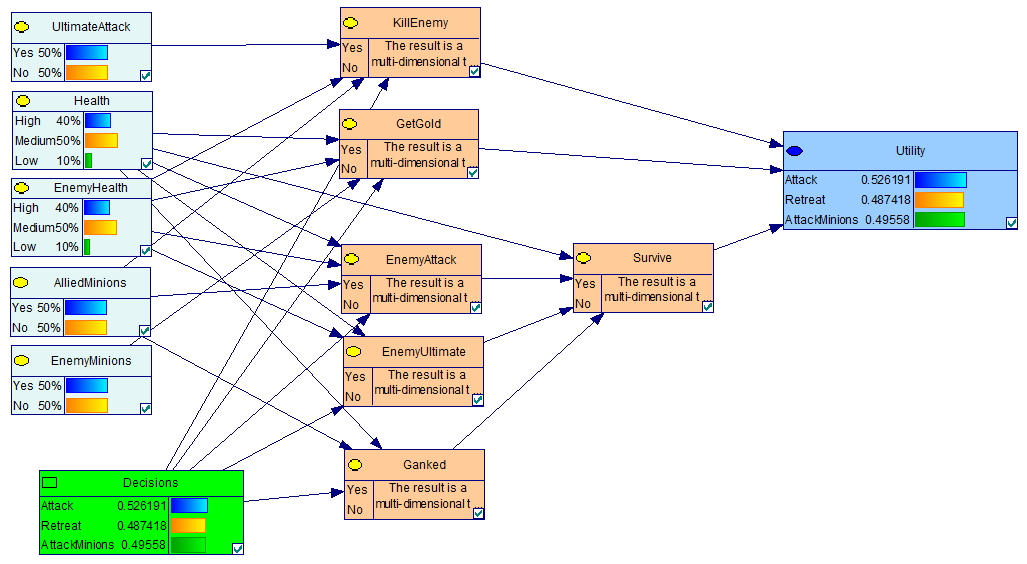
\includegraphics[width=400px]{InfluenceDiagram.PNG}
\caption{Influence diagram}
\end{figure}

The tables to the different variables are too huge to show in this delivery. We have instead chosen to show extracts from two of the tables. This shows how we have modelled the different variables. We can se from Figure~\ref{fig:KillEnemy} how likely we are to kill the enemy given ultimate Attack, enemy Health, allied Minions, and decisions. We see that as long as the enemy has medium health and we have our ultimate we think we have a good possibility to kill the enemy. We also see that it is easier to kill the enemy if we have allied minions as they will help us in the fight. If we don't attack the enemy god we have a 0\% chance of killing him, which is resonable.

\begin{figure}[H]
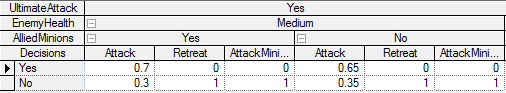
\includegraphics[width=400px]{KillEnemy.PNG}
\caption{Kill Enemy table}
\label{fig:KillEnemy}
\end{figure}

From table~\ref{fig:Survive} we see how likely we are to survive given enemy ultimate, enemy attack, ganked and our health.
We see that that if the enemy use their ultimate, and we are attacked by the enemy or ganked, we are likely to die if we have medium health. We also see that as long as the enemy don't use their ultimate we have a fair chance of surviving.

\begin{figure}[H]
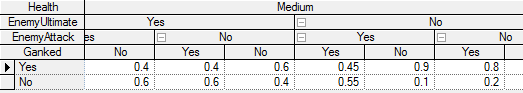
\includegraphics[width=400px]{SurviveTable.PNG}
\caption{Survive table}
\label{fig:Survive}
\end{figure}

\section{Utility function}The utility function is based on how the diffrent outcomes affect the strength of our team and the god we are playing. The bigger the chance that an action will help our team, the better the action is. We have tried to modify the utility function to best represent how much diffrent actions will help the team. The exact numbers for this is of course very complicated and way to much reserch for this assignment, but we are confident that we have pretty good estimations. 

The most important thing is not to die. When you die your team are extremely vulnerable, because they have one more god than your team. You also give gold to the enemy, and loose gold yourself. As long as you stay alive you should be pretty happy. It is not adequate to just stay alive though, you have to get as much gold as you can and try to kill the enemy gods. To kill the enemy god is very good, because it will leave the enemy team in a bad spot and leave you safe. If you can't kill the enemy god and are pretty safe you should just kill minions to get more gold and become stronger.

\begin{table}[H]
\centering
\begin{tabular}{ |c|c|c|c| }

\hline
KillEnemy & Survive & GetGold & Utility \\ \hline
\multirow{4}{*}{Yes} & \multirow{2}{*}{Yes} & Yes & 1 \\ \cline{3-4}
 & & No & 0.8 \\ \cline{2-4}
 & \multirow{2}{*}{No} & Yes & 0.4 \\ \cline{3-4}
 & & No & 0.2 \\ \hline

 \multirow{4}{*}{No} & \multirow{2}{*}{Yes} & Yes & 0.7 \\ \cline{3-4}
 & & No & 0.6 \\ \cline{2-4}
 & \multirow{2}{*}{No} & Yes & 0.05 \\ \cline{3-4}
 & & No & 0 \\ \hline
\end{tabular}
\caption{Utility table}
\end{table}


\section{Verification}
To check that our modelling seems resonable, we have tried different values for our known variables. We see that we can get all the different decisions and that the decision made corresponds well with our initial thoughts. Bellow you can see some of the results we got after testing the model.

\subsection*{Attack minions decision}
UltimateAttack = Yes \\*
Health = High \\*
EnemyHealth = High \\*
AlliedMinions = No \\*
EnemyMinions = Yes \\*

\begin{figure}[H] \centering
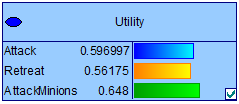
\includegraphics[width=230px]{atkMin.PNG}
\caption{AttackMinion}
\label{fig:atkMin}
\end{figure}

Since both players have high health and we don't have any minons to help us, there is little chance of killing the enemy or get killed. Therefore it seems resonable to kill the enemy minions and get more gold. There is little to gain by attacking the enemy or retreating.

\subsection*{Attack enemy decision}
UltimateAttack = Yes \\*
Health = High \\*
EnemyHealth = Low \\*
AlliedMinions = Yes \\*
EnemyMinions = Yes \\*

\begin{figure}[H] \centering
\includegraphics[width=230px]{atkEnemy.PNG}
\caption{AttackEnemy}
\label{fig:atkEnemy}
\end{figure}

Since we are in a clearly stronger position than your enemy it seems very reasonable to attack him and hope to get a kill. We see that we have high health as well as minions and are not likely to get killed. Since we have our ultimate ready we should also be able to kill him before he gets away.

\subsection*{Retreat decision}
UltimateAttack = No \\*
Health = Low \\*
EnemyHealth = Medium \\*
AlliedMinions = No \\*
EnemyMinions = Yes \\*

\begin{figure}[H] \centering
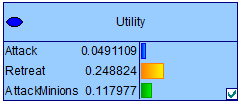
\includegraphics[width=230px]{Retreat.PNG}
\caption{Retreat}
\label{fig:retreat}
\end{figure}

Since we have little health, and the enemy has support from his minions it is best to just retreat. We don't have our ultimate attack so there is not much chance for us to fight back if we are attacked. 

\section{team members' preferences}
We have pretty much the same perception of how the uncertain variables should count. The only diffrence we have encountered is that we have a little diffrent playing styles, where one focus more on killing the enemy and the other focus more on surviving. We have after some discussion come to an agreement where we simply met in the middle.  

\end{document}

